\documentclass[10pt]{article} % Common document class for reports/papers
\usepackage[utf8]{inputenc} % Allows for UTF-8 encoding
\usepackage[left=0.5in, right=1.5in, top=1in, bottom=1in]{geometry} % Sets 1-inch margins all around
\usepackage{multirow} % For complex tables, if needed
\usepackage{array} % For better control of table columns
\usepackage{helvet} % Uses the Helvetica font family
\usepackage{tikz}
\usepackage{amsmath}
\usepackage{amsfonts}
\usepackage{amsthm}

\usepackage{varwidth}

\usepackage{fancyhdr}
\pagestyle{fancy}
\renewcommand{\headrulewidth}{0pt}
\lhead{University of Evansville}
\chead{School of Education}
\rhead{Lesson plan}
\lfoot{SOE Lesson Plan Form}
\cfoot{}
\rfoot{\thepage}

\usepackage{tabularx}
\newcolumntype{Y}{>{\centering\arraybackslash}X}

\usepackage{colortbl}
\usepackage{xcolor}

\renewcommand{\arraystretch}{1.5}

\begin{document}

%\begin{tabularx}{\textwidth}{Y}
  {\large University of Evansville Lesson Plan Format } \\
  \arrayrulecolor{blue} \hline \\
\end{tabularx}


\arrayrulecolor{black} 
\begin{tabularx}{\textwidth}{|X|X|}
  \hline 
  \textcolor{blue}{Name:}          &   \textcolor{blue}{Student ID Number:} \\
  \hline 
  \textcolor{blue}{Course Number:} &   \textcolor{blue}{Instructor Name:} \\
  \hline 
\end{tabularx}
\arrayrulecolor{black} 

\vskip 10pt
  
\begin{tabularx}{\textwidth}{Y}
  {\bf Lesson Overview} \\
\end{tabularx}
\arrayrulecolor{black}


\arrayrulecolor{black} 
\begin{tabularx}{\textwidth}{|X|X|}
  \hline 
  \textbf{Lesson Title:} \\
  
  \hline 
  \textbf{Subject:} \\
  
  \hline 
      {
        \begin{tabularx}{\textwidth}{X|X}
          \hskip -6pt
          \textbf{Duration of Lesson:} & \textbf{Grade Level(s)/Course:} \\
        \end{tabularx}
      } \\
      
      \hline
      
      \textbf{Lesson Description: {\tiny (Describe the primary nature e.g. hands-on, direct instruction, inquiry, project based etc. of the lesson)}} \\
        
        \hline
        
        \textbf{Standards and/or Indicator(s):} {\tiny Cut and paste from IDOE website here. Feel free to replicate the descriptors listed below to include more standards in this section.} \\
        \textbf{Indiana Standard number:} \\
        \textbf{Text:} \\
        \hline
        
        \textbf{Learning Objective(s)/Target:} {\tiny What do I want students to learn and be able to do at the end of the lesson? (I can statements)}
               {\begin{enumerate}
                 \item Lorum
                 \item ipsum
               \end{enumerate}} \\
               \hline
               
               \textbf{Lesson Resources/Technology: } {\tiny (What technology will I use? What technology will students use for this lesson? What resources will you and/or the students need for the lesson – books, mentor texts, etc.)} \\
               \hline
        
               \textbf{Key Vocabulary:} {\tiny List all key vocabulary words that will be taught to help students understand the concepts in the lesson.} \\
               \hline
\end{tabularx}
\arrayrulecolor{black}

\pagebreak

\begin{tabularx}{\textwidth}{|p{0.5in}|X|}
  \hline
  \centerline{\textbf{\large Time}} &  \textbf{\large Instructional Sequence } \\
  \hline
  \textbf{} &  \textbf{\em Introduction/Anticipatory Set:} {\tiny What meaningful activity will engate students, activate prior knowledge, and prepare students for learning objectives} \\
  \hline
  \textbf{} &  \textbf{\em Demonstrate, Build, Apply Knowledge} {\tiny What meaningful activity will engate students, activate prior knowledge, and prepare students for learning objectives} \\
  \hline
  \textbf{} &  \textbf{\em Depth of Knowledge Questions:} {\tiny Essential questions to extend higher level thinking)
} \\
  \hline
  \textbf{} &  \textbf{\em Guided Practice:} {\tiny (Check for understanding prior to independent work; “We do”)} \\
  \hline
  \textbf{} &  \textbf{\em Independent Practice:} {\tiny (Individual practice, learning centers, reading, composing writing; “You do”)} \\
  \hline
  \textbf{} &  \textbf{\em Assessment:} {\tiny (Evaluate level of student understanding. How will I know if students have achieved today’s learning target?)} \\
  \hline
  \textbf{} &  \textbf{\em Wrap Up/Closing Activity/Reflection:} {\tiny (How will I reinforce/revisit the learning objective? Opportunity for formative assessment. Students reflect on evidence of learning – writing, reading, math target. How will we build on this learning?)} \\
  \hline
\end{tabularx}

\vskip 6pt

\begin{small}
\begin{tabularx}{\linewidth}{|p{2.1in}|X|}
  \hline
  \textbf{Differentiation/Accommodations and/or Modifications: } & \\
  \hline
  \textbf{Culturally Responsive Teaching/ Diversity and Inclusion: } & \\
  \hline
\end{tabularx}

\vskip 6pt

\begin{tabularx}{\linewidth}{|X|}
  \hline
  \textbf{Self-Reflection:} \\
  \textbf{My Teaching:} 
  \begin{enumerate}
  \item .
  \item .
  \end{enumerate} \\
  
  \textbf{The Students:}
  \begin{enumerate}
  \item .
  \item .
  \end{enumerate} \\
  
  \textbf{The Lesson:}
  \begin{enumerate}
  \item .
  \item .
  \end{enumerate} \\
  
  \hline
\end{tabularx}
\end{small}

%\begin{tabularx}{\textwidth}{Y}
  {\large University of Evansville Lesson Plan Format 8/29/2025} \\
  \arrayrulecolor{blue} \hline \\
\end{tabularx}


\arrayrulecolor{black} 
\begin{tabularx}{\textwidth}{|X|X|}
  \hline 
  \textcolor{blue}{Name:} Randall Helzerman         &   \textcolor{blue}{Student ID Number:} 0128861 \\
  \hline 
  \textcolor{blue}{Course Number:} EDUC-497-03 2025FA &   \textcolor{blue}{Instructor Name:} Dr. Laura Watkins\\
  \hline 
\end{tabularx}
\arrayrulecolor{black}

\vskip 10pt

\begin{tabularx}{\textwidth}{Y}
  {\bf Lesson Overview} \\
\end{tabularx}
\arrayrulecolor{black}


\arrayrulecolor{black} 
\begin{tabularx}{\textwidth}{|X|X|}
  \hline 
  \textbf{Lesson Title:} \\
  
  \hline 
  \textbf{Subject:} Math\\
  
  \hline 
      {
        \begin{tabularx}{\textwidth}{X|X}
          \hskip -6pt
          \textbf{Duration of Lesson: 80 min} & \textbf{Grade Level(s)/Course:} 8th grade\\
        \end{tabularx}
      } \\
      
      \hline
      
      \textbf{Lesson Description: THE PYTHAGOREAN THEOREM} (in all-caps!)\\
      
      \hline
      
      \textbf{Standards and/or Indicator(s):}\\
      \textbf{Indiana Standard number:} 8.GM.8\\
      \textbf{Text:} Apply the Pythagorean Theorem to determine unknown side lengths in right triangles in real-world and other
      mathematical problems in two dimensions.\\
      \hline
      
      \textbf{Learning Objective(s)/Target:} \\
             {\begin{enumerate}
               \item Students should know what a right triangle is
               \item Students should feel comfortable 
             \end{enumerate}} \\
             \hline
             
             \textbf{Lesson Resources/Technology: } 6 3x5 cards for a Pythagorean triple treasure hunt\\
             \hline
             
             \textbf{Key Vocabulary:} 
             Right angle, right triangle, legs of right triangle, hypoteneus of a right triangle. \\
             \hline
\end{tabularx}
\arrayrulecolor{black}

\pagebreak

\begin{tabularx}{\textwidth}{|p{0.5in}|X|}
  \hline
  \centerline{\textbf{\large Time}} &  \textbf{\large Instructional Sequence } \\
  \hline
  \textbf{5 min} &  \textbf{\em Introduction/Anticipatory Set:}     Draw the following figures on the Promethean board: \\
  10 min & 
  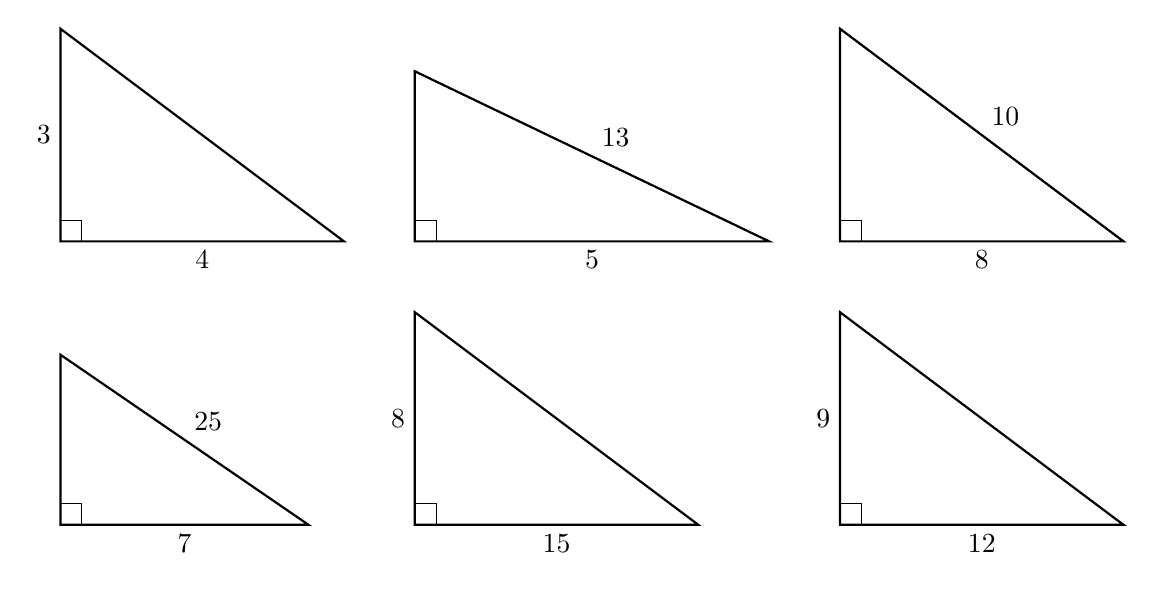
\begin{tikzpicture}[scale=0.9]
    
    % Row 1, Column 1 - Problem 1 (3-4-5 triangle)
    \begin{scope}[shift={(0,0)}]
      \draw[thick] (0,0) -- (4,0) -- (0,3) -- cycle;
      \draw (0.3,0) -- (0.3,0.3) -- (0,0.3);
      \node[below] at (2,0) {4};
      \node[left] at (0,1.5) {3};
    \end{scope}
    
    % Row 1, Column 2 - Problem 2 (5-12-13 triangle)
    \begin{scope}[shift={(5,0)}]
      \draw[thick] (0,0) -- (5,0) -- (0,2.4) -- cycle;
      \draw (0.3,0) -- (0.3,0.3) -- (0,0.3);
      \node[below] at (2.5,0) {5};
      \node[above right] at (2.5,1.2) {13};
    \end{scope}
    
    % Row 1, Column 3 - Problem 3 (6-8-10 triangle)
    \begin{scope}[shift={(11,0)}]
      \draw[thick] (0,0) -- (4,0) -- (0,3) -- cycle;
      \draw (0.3,0) -- (0.3,0.3) -- (0,0.3);
      \node[below] at (2,0) {8};
      \node[above right] at (2,1.5) {10};
    \end{scope}
    
    % Row 2, Column 1 - Problem 4 (7-24-25 triangle)
    \begin{scope}[shift={(0,-4)}]
      \draw[thick] (0,0) -- (3.5,0) -- (0,2.4) -- cycle;
      \draw (0.3,0) -- (0.3,0.3) -- (0,0.3);
      \node[below] at (1.75,0) {7};
      \node[above right] at (1.75,1.2) {25};
    \end{scope}
    
    % Row 2, Column 2 - Problem 5 (8-15-17 triangle)
    \begin{scope}[shift={(5,-4)}]
      \draw[thick] (0,0) -- (4,0) -- (0,3) -- cycle;
      \draw (0.3,0) -- (0.3,0.3) -- (0,0.3);
      \node[below] at (2,0) {15};
      \node[left] at (0,1.5) {8};
    \end{scope}
    
    % Row 2, Column 3 - Problem 6 (9-12-15 triangle)
    \begin{scope}[shift={(11,-4)}]
      \draw[thick] (0,0) -- (4,0) -- (0,3) -- cycle;
      \draw (0.3,0) -- (0.3,0.3) -- (0,0.3);
      \node[below] at (2,0) {12};
      \node[left] at (0,1.5) {9};
    \end{scope}
    
  \end{tikzpicture}  \\

  & Ask the students to write on their whiteboards what the labeled
  sides are for each triangle: Is it the hypoteneus, or a leg? \\
  
  \hline
  
  \textbf{} &

  \textbf{\em Demonstrate, Build, Apply Knowledge} We had a Pythagorean triangle treasure hunt.  At 6 stations around the room there was a problem involving a right triangle, and the solution told the students which station to go to next.  If they arrived back at their first station, they won!  See figure \ref{th_pt} for the cards.\\
  
  \hline
  
  \textbf{} & \textbf{\em Depth of Knowledge Questions:} Had students take out their whiteboards, and list out how many kinds of objects they could see in the room which had right angles.  Let them look around for 5 minutes.

  The students were quite surprised by how many there were.   Some students could name over 50 different kinds of objects (blocks the wall was made of, ceiling tiles, posters on the walls, the walls, etc etc).

  I told them I wanted them to do this exercise because the world they happened to find themselves in is just FULL of right angles, and therefore, right triangles.  And that I wanted them to feel comfortable and safe in their world, and in order to do that, they had to be able to understand their world.   And since their world has so many right angles, a good place to start would be learning the Pythagorean theorem.\\
  
  \hline
  
  \textbf{} & \textbf{\em Guided Practice:} Cold-calling the students, asking them how to identify the variios parts of a right triangle, and how to calculate the lengths of the hypoteneuse.\\
  
  \hline
  
  \textbf{} & \textbf{\em Independent Practice:} Work on some problems from workbook  \\
  
  \hline

  \textbf{} & \textbf{\em Assessment:} We gave an exit ticket to test basic knowledge.\\
  \hline
  
  \textbf{} & \textbf{\em Wrap Up/Closing Activity/Reflection:} N/A\\
  
  \hline
\end{tabularx}
  
\vskip 6pt

\begin{small}
\begin{tabularx}{\linewidth}{|p{2.1in}|X|}
  \hline
  \textbf{Differentiation/Accommodations and/or Modifications: } & Paid more attention to explaining what ``consecutive numbers'' meant.   Most students were not familiar with the word ``consecutive.''\\
  \hline
  \textbf{Culturally Responsive Teaching/ Diversity and Inclusion: } & N/A\\
  \hline
\end{tabularx}

\vskip 6pt

\begin{tabularx}{\linewidth}{|X|}
  \hline
  \textbf{Self-Reflection:} \\
  \textbf{My Teaching:} 
  \begin{enumerate}
  \item After looking at the exit tickets from the first session, it was obvious that I had not done enough explaining what ``consecutive numbers'' were.   I modified my approach and the next session did much better on the exit ticket.
  \item .
  \end{enumerate} \\
  
  \textbf{The Students:}
  \begin{enumerate}
  \item The students really liked the treasure hunt, and they really liked naming out all of the things in the room which had right angles.  
  \item They were amazed that there were so many.  
  \end{enumerate} \\
  
  \textbf{The Lesson:}
  \begin{enumerate}
  \item As noted above, the lesson was a bit thin on explaining what ``consecutive numbers'' were.  
  \end{enumerate} \\
  
  \hline
\end{tabularx}
\end{small}

%\include{lp_sep_2}
%\begin{tabularx}{\textwidth}{Y}
  {\large University of Evansville Lesson Plan Format } 9/3/2025 TO 9/4/2025\\
  \arrayrulecolor{blue} \hline \\
\end{tabularx}


\arrayrulecolor{black} 
\begin{tabularx}{\textwidth}{|X|X|}
  \hline 
  \textcolor{blue}{Name:} Randall Helzerman
  &
  \textcolor{blue}{Student ID Number:} 0128861 \\
  \hline
  
  \textcolor{blue}{Course Number:} EDUC-497-03 2025FA
  &
  \textcolor{blue}{Instructor Name:} Dr. Laura Watkins\\
  \hline
  
\end{tabularx}
\arrayrulecolor{black} 

\vskip 10pt
  
\begin{tabularx}{\textwidth}{Y}
  {\bf Lesson Overview} \\
\end{tabularx}
\arrayrulecolor{black}


\arrayrulecolor{black} 
\begin{tabularx}{\textwidth}{|X|X|}
  \hline
  
  \textbf{Lesson Title:} \\
  \hline
  
  \textbf{Subject:} Math\\
  \hline
  
  {\begin{tabularx}{\textwidth}{X|X}
      \hskip -6pt
      \textbf{Duration of Lesson:} & \textbf{Grade Level(s)/Course:}
      8th grade\\
  \end{tabularx}} \\
  \hline
  
  \textbf{Lesson Description: {\tiny (Describe the primary nature
      e.g. hands-on, direct instruction, inquiry, project based
      etc. of the lesson)}} \\
  \hline
  
  \textbf{Standards and/or Indicator(s):} {\tiny Cut and paste from
    IDOE website here. Feel free to replicate the descriptors listed
    below to include more standards in this section.} \\
  
  \textbf{Indiana Standard number:} \\
  
  \textbf{Text:} \\
  
  \hline
  
  \textbf{Learning Objective(s)/Target:} {
    \begin{enumerate}
    \item I can solve simple equations using squares and cubes.
    \item I know how to use the pythagorean theorem to find the length
      of the hypotenuse.
    \end{enumerate}
  }   \\
  \hline
  
  \textbf{Lesson Resources/Technology: } Promethean board \\
  \hline
  
  \textbf{Key Vocabulary:} \\ square, square root, cube, cube root,
  consecutive, hypotenuse, pythagorean theorem, operator, inverse
  operator. \\
  \hline
  
\end{tabularx}
\arrayrulecolor{black}

\pagebreak

\begin{tabularx}{\textwidth}{|p{0.5in}|X|}
  \hline
  
  \centerline{\textbf{\large Time}} &  \textbf{\large Instructional Sequence } \\
  
  \hline
  
  \textbf{} & \textbf{\em Introduction/Anticipatory Set:} Write the following simple equtions on the whiteboard:
  \[
    \begin{array}{c c c}
      c^{2}=15  & c^{2}=35  & c^{2}=8 \\
      c^{2}=27  & c^{2}=12  & c^{2}=17 \\
    \end{array} \]

   and ask the students to solve.  Then go over their answers. \\
  \hline
  
  \textbf{} & \textbf{\em Demonstrate, Build, Apply Knowledge}  N/A\\
  \hline
  
  \textbf{} & \textbf{\em Depth of Knowledge Questions:} N/A \\
  \hline
  
  \textbf{} & \textbf{\em Guided Practice:}   Worked a few problems on the study guide on the board.\\
  \hline
  
  \textbf{} & \textbf{\em Independent Practice:}  Study guide for test tomorrow. \\
  \hline
  
  \textbf{} & \textbf{\em Assessment:}  Test tomorrow \\
  \hline
  
  \textbf{} & \textbf{\em Wrap Up/Closing Activity/Reflection:} N/A \\
  \hline 
\end{tabularx}

\vskip 6pt

\begin{small}
  \begin{tabularx}{\linewidth}{|p{2.1in}|X|}
    \hline
    \textbf{Differentiation/Accommodations and/or Modifications: } & N/A\\
    \hline
    \textbf{Culturally Responsive Teaching/ Diversity and Inclusion: } & N/A\\
    \hline
  \end{tabularx}
  
  \vskip 6pt

  \begin{tabularx}{\linewidth}{|X|}
    \hline
    \textbf{Self-Reflection:} \\
    \textbf{My Teaching:} 
    \begin{enumerate}
    \item Made a critical mistake: emphasized that we want the answer to
      be consecutive whole numbers, but then explained how to solve the
      problems by advertint to perfect squares, which are not
      consecutive.  This confused a lot of students.  Fortunatey I fixed
      in in the subsequent presentations.
    \end{enumerate} \\
    
    \textbf{The Students:}
    \begin{enumerate}
    \item The students have a rather limited vocabulary, and we have to
      be sensitive to that.  The word ``consecutive'' was new to them,
      and it took a few days for them to wrap their heads around it.
    \end{enumerate} \\
2    
    \textbf{The Lesson:}
           \begin{enumerate}
             \item We are trying to adhere to the prescribed lessons as much as
               possible, but this particular unit did not seem to have very
               effective structure.  To the students, it just seem like a grab-bag of ad-hoc techniques.
             \item They are not in algebra class, but yet we are teaching them
               bits and pieces of algebra in order for them to be able to solve
               the problems.   It seems like presenting the rules for, say, canceling a square root with a square, would be easier to understand as part of a larger system of canceling addition with subtraction, etc.  
           \end{enumerate} \\
           
           \hline
\end{tabularx}
\end{small}

\begin{tabularx}{\textwidth}{Y}
  {\large University of Evansville Lesson Plan Format } \\
  \arrayrulecolor{blue} \hline \\
\end{tabularx}


\arrayrulecolor{black} 
\begin{tabularx}{\textwidth}{|X|X|}
  \hline 
  \textcolor{blue}{Name:} Randall Helzerman
  &
  \textcolor{blue}{Student ID Number:} 0128861 \\
  \hline
  
  \textcolor{blue}{Course Number:} EDUC-497-03 2025FA
  &
  \textcolor{blue}{Instructor Name:} Dr. Laura Watkins\\
  \hline
  
\end{tabularx}
\arrayrulecolor{black} 

\vskip 10pt
  
\begin{tabularx}{\textwidth}{Y}
  {\bf Lesson Overview} \\
\end{tabularx}
\arrayrulecolor{black}


\arrayrulecolor{black} 
\begin{tabularx}{\textwidth}{|X|X|}
  \hline
  
  \textbf{Lesson Title:} \\
  \hline
  
  \textbf{Subject:} Math\\
  \hline
  
  {\begin{tabularx}{\textwidth}{X|X}
      \hskip -6pt
      \textbf{Duration of Lesson:} & \textbf{Grade Level(s)/Course:} 8th grade\\
  \end{tabularx}} \\
  \hline
  
  \textbf{Lesson Description: {\tiny (Describe the primary nature
      e.g. hands-on, direct instruction, inquiry, project based
      etc. of the lesson)}} \\
  \hline
        
  \textbf{Standards and/or Indicator(s):} {\tiny Cut and paste from
    IDOE website here. Feel free to replicate the descriptors listed
    below to include more standards in this section.} \\
  
  \textbf{Indiana Standard number:} \\
  
  \textbf{Text:} \\
  
  \hline
        
  \textbf{Learning Objective(s)/Target:} {\tiny What do I want
    students to learn and be able to do at the end of the lesson? (I
    can statements)}
  
  {\begin{enumerate}
    \item Lorum
    \item ipsum
  \end{enumerate}} \\
  \hline
               
  \textbf{Lesson Resources/Technology: } {\tiny (What technology will
    I use? What technology will students use for this lesson? What
    resources will you and/or the students need for the lesson –
    books, mentor texts, etc.)} \\
  \hline
        
  \textbf{Key Vocabulary:} {\tiny List all key vocabulary words that
    will be taught to help students understand the concepts in the
    lesson.} \\ \hline
  
\end{tabularx}
\arrayrulecolor{black}

\pagebreak

\begin{tabularx}{\textwidth}{|p{0.5in}|X|}
  \hline
  \centerline{\textbf{\large Time}} &  \textbf{\large Instructional Sequence } \\
  \hline
  
  \textbf{} & \textbf{\em Introduction/Anticipatory Set:} {\tiny What
    meaningful activity will engate students, activate prior
    knowledge, and prepare students for learning objectives} \\
  \hline
  
  \textbf{} & \textbf{\em Demonstrate, Build, Apply Knowledge} {\tiny
    What meaningful activity will engate students, activate prior
    knowledge, and prepare students for learning objectives} \\
  \hline
  
  \textbf{} & \textbf{\em Depth of Knowledge Questions:} {\tiny
    Essential questions to extend higher level thinking) } \\
  \hline
  
  
  \textbf{} &  \textbf{\em Guided Practice:} {\tiny (Check for understanding prior to independent work; “We do”)} \\
  \hline
  \textbf{} &  \textbf{\em Independent Practice:} {\tiny (Individual practice, learning centers, reading, composing writing; “You do”)} \\
  \hline
  \textbf{} &  \textbf{\em Assessment:} {\tiny (Evaluate level of student understanding. How will I know if students have achieved today’s learning target?)} \\
  \hline
  \textbf{} &  \textbf{\em Wrap Up/Closing Activity/Reflection:} {\tiny (How will I reinforce/revisit the learning objective? Opportunity for formative assessment. Students reflect on evidence of learning – writing, reading, math target. How will we build on this learning?)} \\
  \hline
\end{tabularx}

\vskip 6pt

\begin{small}
\begin{tabularx}{\linewidth}{|p{2.1in}|X|}
  \hline
  \textbf{Differentiation/Accommodations and/or Modifications: } & \\
  \hline
  \textbf{Culturally Responsive Teaching/ Diversity and Inclusion: } & \\
  \hline
\end{tabularx}

\vskip 6pt

\begin{tabularx}{\linewidth}{|X|}
  \hline
  \textbf{Self-Reflection:} \\
  \textbf{My Teaching:} 
  \begin{enumerate}
  \item .
  \item .
  \end{enumerate} \\
  
  \textbf{The Students:}
  \begin{enumerate}
  \item .
  \item .
  \end{enumerate} \\
  
  \textbf{The Lesson:}
  \begin{enumerate}
  \item .
  \item .
  \end{enumerate} \\
  
  \hline
\end{tabularx}
\end{small}


\end{document}
